\documentclass[../ala_hataile.tex]{subfiles}
\begin{document}
	\clearpage
	
\includepdf[pages=28-29, pagecommand={}]{sisasivut_19062018.pdf}
	\raggedbottom
	\twocolumn[\section{Kiehtova TKT} { \small \itshape ``Yleensä tuoreella tietojen\-käsittely\-tieteen opiskelijalla (eli käpistelijällä) ei ole juuri minkäänlaista käsitystä siitä, mitä tietojen\-käsittely\-tiede (eli TKT) tosiasiassa on. Moni kuvittelee tietojen\-käsittely\-tieteen olevan ohjelmointia, mitä se ei suinkaan ole. Ohjelmointi on TKT:ssä vain yksi -- joskin tärkeä työväline.''}\vspace{0.5cm}]
	
	\subsection*{Tietojen\-käsittely\-tiede tieteenä}
	Eräs tyypillinen yhden
	virkkeen tiivistelmä on, että tietojen\-käsittely\-tieteessä
	tutkitaan, mitä voidaan automatisoida
	tehokkaasti. Hieman pidemmin
	ilmaistuna tietojen\-käsittely\-tieteessä ollaan
	kiinnostuneita siitä, mihin voidaan löytää
	luotettava, tehokas ja automatisoitu ratkaisu.
	
	Matematiikassa riittää todistaa, että
	ongelmaan on olemassa ratkaisu. Teoreettisessa
	tietojen\-käsittely\-tieteessä tämä
	ratkaisu on lisäksi pystyttävä löytämään
	tehokkaasti. Tietojen\-käsittely\-tieteen sovelluksissa,
	esimerkiksi ohjelmistotuotannossa,
	tämäkään ei riitä, vaan tehokas menetelmä
	on lisäksi pystyttävä toteuttamaan
	luotettavasti ja tehokkaasti. Ehkäpä siis
	voidaankin sanoa, että tietojen\-käsittely\-tieteessä
	on kysymys luotettavien ja tehokkaiden
	ratkaisujen löytämisestä erilaisiin
	ongelmiin.
	
	Suurin osa tietotekniikka-alan töistä
	liittyy tavalla tai toisella ohjelmistokehitykseen,
	mikä tarjoaa mitä erilaisimpia
	työmahdollisuuksia esimerkiksi ohjelmoinnista,
	ohjelmistosuunnittelusta tai
	tietojenkäsittelyn teoriasta kiinnostuneille.
	Tietojen\-käsittely\-tiede tarjoaa
	monenlaisia kursseja mm.\,kaikista edellä
	mainituista tietojenkäsittelyn osa-alueista.
	Käytännössä tietojen\-käsittely\-tiede antaa
	valmiudet mille tahansa alalle, jossa ongelmanratkaisu
	on keskeisessä asemassa. Nykyään ongelmien ratkaisuun vieläpä
	useimmiten liittyy tavalla tai toisella tietotekniikka.
	
	Tietojen\-käsittely\-tiede on informaation
	tuottamiseen ja koneelliseen käsittelyyn
	perustuva ala. Tietojen\-käsittely\-tieteelliselle
	ajattelulle on tyypillistä, että ongelmat
	jaetaan osaongelmiin, jotka ovat tarpeeksi
	yksinkertaisia ratkaistavaksi. Tämä saattaa
	kuulostaa suoraviivaiselta, mutta oppiessaan
	todella soveltamaan tätä ajattelutapaa
	arkipäivän elämässä, huomaa saaneensa
	jotain todella arvokasta. Monimutkaisen
	kokonaisuuden hallinta ja olennaisen hahmottaminen
	ovat keskeisimpiä taitoja tietojen\-käsittely\-tieteessä.
	
	TKT:n opiskelussa tekijän oma osallistuminen
	on ensisijaisen tärkeää, sillä useimmiten pelkkä
	luennoilla istuminen ei riitä asioiden sisäistämiseen. 
	Keskeistä on, että TKT:n opiskelussa esiin tulevia asioita
	pitää ymmärtämisen lisäksi osata myös
	soveltaa. Opetettavien asioiden ulkoa opiskelu
	ei riitä, joskin tarkka perus\-totuuksien
	osaaminen auttaa opiskelun eri vaiheissa. Kursseja 
	käydessään kannattaakin ottaa harjoitusryhmistä kaikki irti.
	
	Tietojenkäsittelyn ongelmiin on harvoin
	olemassa yksittäisiä oikeita ratkaisuja; ratkaisutapoja
	on useita ja vastaukset voivat
	olla hyvinkin erilaisia. Sen takia tietojenkäsittelyssä
	ei ole aina olemassa oikeaa
	vastausta tuottavaa kaavaa tai prosessia,
	jolla ongelma pystytään ratkaisemaan. Ongelmien
	ratkaisemisen tapauskohtaisuus
	johtuu osaksi siitä, että tietojen\-käsittely\-tiede
	on nuori tieteenala ja osaksi siitä, että
	tietojen\-käsittely\-tieteen ongelmat esiintyvät
	eri paikoissa eri muodossa. Monien mielestä
	mielenkiintoisia ovat myös ongelmat,
	joihin ei ratkaisua, ainakaan toistaiseksi,
	ole olemassa.
	
	\subsection*{Teoriaa ja käytäntöä}
	Helsingin yliopiston tietojen\-käsittely\-tieteen opetus\-sunnitelma on
	alan teoreettisin Suomen monialaisissa
	yliopistoissa. Varsin yleistä onkin kuulla
	vaatimuksia, että opetuksessa pitäisi vähentää
	teoriaa ja lisää käytännön osaamista.
	Tällaiset vaatimukset eivät ole ominaisia
	vain tietojen\-käsittely\-tieteelle tai Helsingin
	yliopiston tietojen\-käsittely\-tieteen opetukselle.
	Vastaavaa kuulee miltei kaikkialla
	ja usein nimenomaan suhteellisen nuorten
	tieteenharjoittajien suusta. Kun opinnoissa
	on sitten edetty pidemmälle, vaatimukset
	usein laantuvat.
	
	Kysymys lienee siitä, että teoriasta on
	usein vaikea saada otetta, jos ei ole myös
	riittävää käytännön osaamista perspektiiviä
	antamassa. Toisaalta kysymys on
	usein myös vääristä odotuksista siitä, mistä
	yliopisto-opiskelussa oikein on kysymys.
	Yliopisto ei opeta suoraan työelämässä
	tarvittavia taitoja vaan ennemminkin valmiuksia,
	joilla sellaiset taidot voi hankkia.
	Vaikka lyhyellä aikavälillä käytännön
	taitojen opettelu olisikin hyödyllisempää,
	vanhenevat sellaiset taidot pian nopeasti
	kehittyvillä aloilla. Riittävät teoreettiset
	valmiudet sen sijaan helpottavat kehityksen
	kelkassa pysymistä, kun uusia asioita ei
	tarvitse opetella alusta alkaen, vaan niiden 
	tunnistaa toimivan jonkin yleisemmän periaatteen
	mukaisesti. Tietojen\-käsittely\-tieteen
	perimmäiset ongelmat eivät ole juurikaan,
	jos ollenkaan, aikojen saatossa muuttuneet.
	
	Moni aloitteleva opiskelija hieman virheellisesti
	ajattelee, että vaikeimpia ongelmia
	ovat juuri matemaattiset pulmat tai
	tekniset rajoitteet. Esimerkiksi ohjelmistotuotannossa
	keskeisimmät ongelmat liittyvät
	ohjelmistoprosesseihin, johtamiseen ja
	asiakkaan kanssa toimimiseen. TKT:lle
	ei tosin kannata tulla silläkään asenteella,
	ettei ``käpistelijän tarvitse osata ohjelmoida''.
	Tällaisille henkilöille oikeampi paikka
	lienee jokin kauppakorkeakoulu.
	
	Tietojen\-käsittely\-tieteen tutkinto\-vaatimuksissa
	ei ole käytännön ohjelmointi- tai
	muiden taitojen opettelua alun jälkeen.
	Opiskelijan oletetaan itse täydentävän tällaisia
	taitojaan tarpeen mukaan, vaikka tätä
	ei missään suoraan mainitakaan. Uuden
	ohjelmointikielen opettelu ei loppujen lopuksi
	ole kovinkaan suuri ponnistus, kunhan
	ohjelmointi\-kokemus hieman karttuu.
	Tämä taas onnistuu paremmin työelämässä
	tai harrastusprojekteissa kuin tekemällä
	harjoitustyötä harjoitustyön perään. Kiinnostus
	opiskelualaa kohtaan myös opintojen
	ulkopuolella lienee asia, jota yliopisto-opiskelijalta voidaan edellyttää. Ilman
	sitäkin tutkinnon voi toki suorittaa, mutta
	silloin taidot jäävät melko vajavaisiksi.
	Tietojen\-käsittely\-tieteen opiskelijan opiskelun
	ja vapaa-ajan raja on useimmiten hyvin
	häilyvä.
	
	\subsection*{Matematiikkaa ja tilastotiedettä}
	Tietojen\-käsittely\-tieteen opiskelijan
	tutkintoon kuuluu pakollisena osana
	matematiikkaa tai menetelmätieteitä
	(=~matematiikkaa sekä tilastotiedettä). Osittain
	tämä johtuu historiallisista syistä -- tietojen\-käsittely\-tiede
	erkani matematiikasta
	itsenäiseksi tieteeksi joitain vuosikymmeniä
	sitten. Osittain taas kysymys on siitä,
	että tietojen\-käsittely\-tiedettä opiskeltaessa
	ja harjoitettaessa välillä tarvitsee matematiikkaa.
	
	Toisin kuin vaikkapa fyysikot, käpistelijät
	opiskelevat matematiikkaa enimmäkseen
	samasta syystä kuin matemaatikot
	itsekin: oppiakseen matemaattista ajattelua
	eikä niinkään menetelmiä ja työkaluja.
	Vaikka lähes mille tahansa matematiikan
	haaralle löytyy sovelluskohteita tietojen\-käsittely\-tieteestä,
	on olennaisempaa kuitenkin
	tulla toimeen formalismien ja matemaattisten
	todistusten kanssa. Formaali
	päättely, matemaattinen todistaminen ja
	ohjelmointi ovat kaikki loppujen lopuksi
	varsin samankaltaisia asioita, vaikka yhteyttä
	niiden välillä voikin olla vaikea nähdä
	ennen kuin on tutustunut kaikkiin näihin
	pintaa syvemmältä.
	
	Matematiikan kursseista Johdatus yliopistomatematiikkaan
	on kaikille käpistelyn opiskelijoille
	pakollinen. Logiikan,
	todennäköisyyslaskennan ja tilastollisen
	päättelyn opiskelu on hyödyllistä, sillä ne
	tarjoavat välineitä ajatteluun ja päättelyyn.
	Raja-arvot, Differentiaalilaskenta, Sarjat,
	Integraalilaskenta sekä Lineaarialgebra ja
	matriisilaskenta~I taas ovat hyödyllisiä lähinnä
	siksi, että ne ovat matematiikan opiskelijoille
	pakollisia ensimmäisen vuoden kursseja. 
	Tämän vuoksi niillä opetetaan kurssien 
	varsinaisen sisällön lisäksi
	myös matematiikan opiskelua. Lisäksi
	niiden tiedot saatetaan olettaa tunnetuiksi
	myöhemmillä kursseilla, vaikka tätä ei olisi
	erikseen mainittukaan, koska ``kaikkihan
	ne ovat kuitenkin käyneet''.
	
	\subsection*{Tietojen\-käsittely\-tieteen osasto}
	
	\subsubsection*{Käyttäjätunnukset}
	Kaikki käpistelijät saavat käyttäjä\-tunnuksen
	osaston mikro\-verkkoon
	ja näin ollen pääsevät käyttämään osaston
	mikro\-luokkien tieto\-koneita. Tunnuksia
	myöntää yllä\-pito, joka majailee
	Exactumin 2.\,kerroksen A-siivessä. Myös
	toisten koulutus\-ohjelmien opiskelijat saavat pyytäessään
	käyttäjä\-tunnuksia muun muassa kurssien
	harjoitus\-töiden tekemistä varten. CS-tunnusten hankkimis\-ohjeet löytyvät osoitteesta:
	\\\url{www.cs.helsinki.fi/activate}
	
	Kaikissa opiskelijoiden käytössä olevissa
	koneissa on Linux-käyttöjärjestelmä.
	Osassa koneista on myös Windows. Käyttöjärjestelmät
	on asennettu siten, että käyttäjät
	pääsevät käsiksi verkkolevyllä sijaitseviin
	tiedostoihinsa sekä Windowsista että Linuxista.
	
	\subsubsection*{Muoviavain}
	Opiskelijat voivat saada 25~euron panttia
	vastaan käyttöönsä ns.\,muovi\-avaimen
	eli magneetti\-avaimen, jolla pääsee osaan
	osaston mikro\-luokista auki\-olo\-ajoista 
	riippumatta, pois lukien klo 01--07. 
	Tietojen\-käsittely\-tieteen osaston myöntämällä
	opiskelija-avaimella pääsee ympäri\-vuoro\-kautisesti myös
	opiskelijahuone Gurulaan.
	
	Muoviavainta anottaessa on täytettävä
	haku\-lomake, joka löytyy Help\-deskin sivuilta.
	Tarkemmat ohjeet muovi\-avaimen
	hakemiseen löytyvät
	osoitteesta \url{helpdesk.it.helsinki.fi/ohjeet/muut-ohjeet/yokayttoavaimet}
	
	\subsubsection*{Opiskelijahuone Gurula}
	Opiskelijahuone Gurula sijaitsee
	Exactumin pohjakerroksessa. Sen osoite
	on DK115. Gurula on myös TKO-älyn,
	tietojen\-käsittely\-tieteen opiskelijoiden ainejärjestön,
	koti, päämaja ja vaelluskohde,
	jonne opiskelijat vaeltavat toisinaan myös
	vapaa-aikanaan. Niinpä siellä voi esimerkiksi
	liittyä ainejärjestön jäseneksi tai ostaa
	TKO-äly-tuotteita, kuten haalarit, haalarimerkkejä,
	laulukirjan tai aina yhtä tyylikkään
	mustan t-paidan tai hupparin. Gurulassa toimii
	TKO-älyn ympärivuorokautinen ruokavälitys,
	joka on nälkäisen opiskelijan pelastus
	silloin, kun ruokalat eivät täytä asiakkaittensa
	vatsoja.
	
	Gurulaan tilataan lehtiä, kuten Aku Ankka, 
	Hesari, Wired ja Skrolli. Lehtien lisäksi Gurulassa on
	usein ihmisiä, joita kiinnostaa esimerkiksi
	pelata Gurulassa olevia lautapelejä. Gurulan
	vieressä yökäytössä olevalla alueella
	on tietotekniikkaosaston mikroluokkia
	sekä WC, mikä tarjoaa mahdollisuuden
	viettää aikaa Exactumissa riippumatta
	turhan paljon vuorokauden vaihtumistahdista
	ulkomaailmassa.
	
	\subsection*{Opiskelijoiden sähköpostilista}
	Tälle listalle kannattaa liittyä. Listalle
	tulee muutaman kerran vuodessa viesti
	esimerkiksi
	kurssi-ilmoittautumisten alkamisesta
	ja muusta oleellisesta. Näin sinä
	saat tarpeellisen tiedon opiskeluun liittyvistä
	tapahtumista myös sähköpostiisi.
	
	Ohjeet listalle liittymiseen löytyvät osoitteesta
	\url{www.cs.helsinki.fi/opiskelu/opiskelijoiden-s-hk-postilista}.
	
	\subsection*{Muista erityisesti}
	Helsingin yliopiston
	tietojen\-käsittely\-tieteen uusille opiskelijoille
	suunnattu FuksiWiki, josta löytyy näiden
	tekstien lisäksi paljon muuta käytännönläheistä
	informaatiota: \url{https://fuksiwiki.tko-aly.fi}
	
	Ainejärjestömme TKO-älyn nettisivut,
	jotta et missaisi niitä ``hieman'' rennompia
	tapahtumia. Sivujen osoite on \url{https://www.tko-aly.fi}
	
	\vspace{0.5cm}
	\noindent\textsc{Anssi Syrjäsalo}\\
	\textsc{Piia Hartikka}\\
	\textsc{Miia Rämö}
	
	\twocolumn[\section{Tietojen\-käsittely\-tieteen opinto-opas}]
	
	\subsection*{Tutkinnot ja erikoistumislinjat}
	
	Luonnontieteiden kandidaatin tutkinnossa
	ei vielä kovin paljon pääse erikoistumaan,
	vaan kaikille yhteiset opinnot
	täyttävät valtaosan tutkinnosta. LuK-vaiheessa
	kaikki ovet eivät vielä ole opiskelijalle
	auki, koska syventävillä
	kursseilla vaaditaan yleensä vankat perustiedot
	opetettavasta aiheesta. Suositeltavaa
	tietysti olisi suorittaa LuK-tutkinto pois
	alta mahdollisimman nopeasti, jotta voisi
	sukeltaa niihin ``itselle oikeasti mielenkiintoisiin
	asioihin''.
	\begin{figure}[b]
		\centering
		
\includegraphics[width=\columnwidth]{avainkone.png}
	\end{figure}
	
	Useimmiten motivaatio alkaa romahtaa
	kun LuK-tutkinnosta on suoritettu noin
	kaksi kolmasosaa. Näin sattuessa kannattaa
	ehdottomasti harkita syventävien opintojen
	suorittamista puuttuvien LuK-opintojen
	ohessa. Tällainen menettely on toiminut
	monelle hajonneelle sielulle uutena motivaation
	lähteenä. Lisäksi syventävien
	opintojen läpäiseminen innostanee myös
	tulevien FM-opintojen suorittamiseen. TKT:llä
	on ihan oikeakin haaste estää ihmisiä
	karkaamasta LuK-tutkinnon jälkeen
	työelämään. Ohimennen mainittakoon, että
	tutkintoon ei sisälly enää myöskään työharjoittelua.
	Sitäkin kokeiltiin joskus, mutta
	suurin osa opiskelijoista ei enää palannutkaan
	hyväpalkkaisesta työharjoittelusta
	opiskelemaan.
	
	Omaa erikoistumislinjaa ei tarvitse heti
	päättää. Maisterivaiheessa voi tutkiskella
	erilaisia valmistumisprofiileja, ja kursseja
	voi ja kannattaakin lukea eri linjoilta ristiin.
	Valmistumisella ei rajauksista huolimatta
	ole niin tulipalokiire, ettäkö vain pakolliset
	pahat sisältävä putkitutkinto olisi paras
	vaihtoehto. Niin kauan kuin opiskelu maistuu,
	kannattaa käydä yleensä ottaen mielenkiintoisilta
	tuntuvilla kursseilla -- kun sitten
	aikanaan valmistumisen myötä menettää
	opinto-oikeutensa, hankaloituu opiskelukin
	tuntuvasti. Maisteriopinnoissa käy helposti
	niin, että kun opintoja on aikansa suorittanut,
	huomaa opetus\-suunnitelman täyttyvän
	yhdellä tai useammalla erikoistumislinjalla,
	ja mielessäkin pyörii gradun aihe, joka
	sopisi jollekin näistä linjoista.
	
	Tietojenkäsittelytieteen kandiohjelmasta jatketaan pääasiassa Tietojenkäsittely\-tieteen tai Data\-tieteen maisteri\-ohjelmaan. Tietojen\-käsittely\-tieteen maisteriohjelman sisällä opinto\-suuntia on kolme: Algoritmit, Hajautetut järjestelmät ja tieto\-liikenne sekä Ohjelmisto\-järjestelmät.
	Linjojen sisällöt ovat suunnilleen
	seuraavat:
	
	\textbf{Algoritmien opintosuunta (Alko)}: Jos kandikursseista sytytti Tietorakenteet, Laskennan mallit tai Johdatus tekoälyyn, Algoritmien opintosuunta voisi olla sinun valintasi. Algoritmien opintosuunta tutkii tehokkaita algoritmeja sekä niiden käyttöä.
	
	\textbf{Hajautettujen järjestelmien ja tieto\-liikenteen opinto\-suunta (Hajatili)}: Opinnot käsittelevät kiinteiden verkkojen ja mobiili\-verkkojen suunnittelua ja hallintaa sekä niiden päälle rakentuvia palveluita. Erityisinä fokuksina ovat hajautetut järjestelmät, interaktiiviset järjestelmät sekä järjestelmien mukautuminen muuttuvaan toiminta\-ympäristöön.
	
	\textbf{Ohjelmistojärjestelmät}: Opintosuunta keskittyy suurten ja monimutkaisten ohjelmistojärjestelmien tuottamisen tarkasteluun tutkimalla ohjelmistoprosesseja, ryhmädynamiikkaa ja ohjelmiston laatua sekä niiden uudelleenkäyttöä.
	
	\textbf{Datatieteen maisteriohjelma}: Datatieteen maisteriohjelma käsittelee koneoppimisen, hajautetun laskennan ja tilastotieteen metodeja. Voit joko oppia kehittämään uusia metodeja tai soveltamaan aiemmin tunnettuja metodeja uusissa tilanteissa.
	\begin{figure}[b]
		\centering
		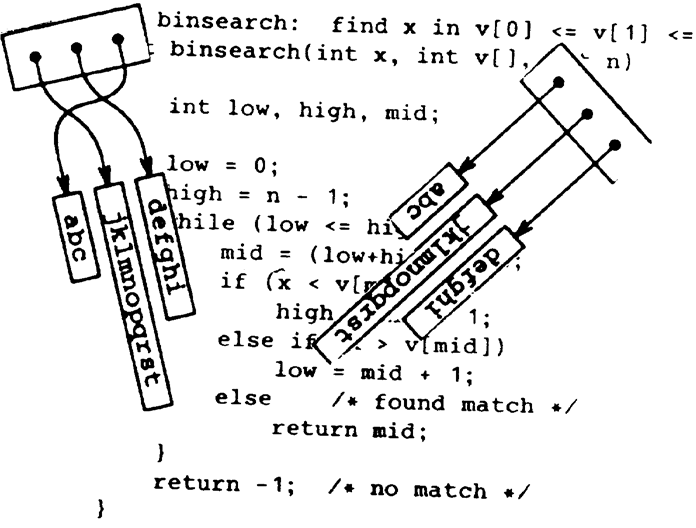
\includegraphics[width=\columnwidth]{vanhaakoodia.png}
	\end{figure}
	
	\subsubsection*{Tutkijalinja}
	Tutkijalinja on löyhä ryhmä ihmisiä,
	joista ainakin opintojen alkuvaiheessa tutkijan
	ura on vaikuttanut hyvältä idealta.
	Tyypillisesti väki on painottunut algoritmien
	ja koneoppimisen suuntaan, muilla
	linjoilla tutkijaksi herätään yleensä myöhemmin.
	
	Tutkijalinjalle pyritään ensimmäisen
	vuoden kevätlukukauden lopussa, mutta
	karsinta ei ole ainakaan yleensä ollut kovin
	tiukka. Aikaisemmin linjan toiminta
	keskittyi siihen, että tutkijalinjalaisilla oli
	2.\,ja 3.\,vuonna kaikille pakollisena olevassa
	opettajatuutoroinnissa oma ryhmänsä,
	joka toimii hiukan omalaatuisemmin kuin
	keskimääräinen opettajatuutorointiryhmä.
	Jotain vastaavaa lienee luvassa tulevaisuudessakin.
	
	Linjasta saatavat konkreettiset edut
	vaihtelevat vuodesta toiseen. Toisinaan
	on saattanut saada kannettavan
	tietokoneen monivuotiseen lainaan, toisinaan
	taas mikroluokkia rauhallisemman
	työskentely-ympäristön. Kesäisin linjalaiset
	saattavat päästä käymään lähialueilla
	olevissa tieteellisissä konferensseissa,
	mikä mahdollisuus kannattaa ehdottomasti
	hyödyntää. Matkailu avartaa ja konferenssimatkailu
	eritoten. Urhealla tutkijanalulla
	tosin voi alkaa kunto pettää viikon edetessä,
	kun jälkilöylybaarista ei tietenkään voi
	lähteä ennen puoltayötä, vaikka seuraavana päivänä olisi taas kahdeksan tuntia esitelmiä
	aamuyhdeksästä alkaen.
	
	Tutkijalinja toimii myös tehokkaana
	rekrytoitumiskanavana tutkimusapulaisen
	töihin; tutkijalinjalaiset ovat
	jo valmiiksi osoittaneet kiinnostusta tutkimukseen,
	joten he ovat haluttua tavaraa
	kun tutkimusryhmät kaipaavat lisävahvistusta.
	
	\subsubsection*{Tärkeitä päivämääriä}
	Ajan myötä saatat huomata, että tärkeät
	päivämäärät pysyvät samanlaisina vuodesta
	toiseen. Ihmiset ovat luonnostaan laiskoja
	eivätkä jaksa yleensä muuttaa asioita
	pelkästä muuttamisen ilosta.
	Niinpä kannattaakin opetella ajoissa,
	mitä missäkin välissä vuotta
	tapahtuu. Opetusohjelmat ilmestyvät, kursseille
	voi ilmoittautua ja opetusperiodit alkavat
	ja päättyvät aina suunnilleen samaan
	aikaan. Kun nämä ajat sisäistää, elämä
	yleensä helpottuu, kun asiat eivät
	enää tule eteen yllättäen.
	
	\subsubsection*{Ohjeita ja sääntöjä}
	Nyrkkisääntö on, että omatoimiseen
	opiskeluun pitäisi varata vähintään yhtä
	paljon aikaa kuin ohjattuun. Toisaalta taas
	sanotaan, että yksi opintopiste vastaa noin
	27~työtuntia. Molemmat näistä ovat keskimäärin
	totta, vaikka vaihtelua onkin paljon
	niin opiskelijoiden kuin opintojaksojenkin
	välillä. Kannattaa joka tapauksessa aloittaa
	opinnot varovaisesti ennen kuin oppii
	tuntemaan omat kykynsä ja yliopisto-opintojen
	vaatimustason -- sekä muistaa, että
	vaatimukset kasvavat opintojen edetessä.
	Mallilukujärjestyksen mukainen 30~op lukukaudessa
	nimittäin edellyttää kokopäiväistä
	työtä keskimääräiseltä ja kohtalaisen
	motivoituneelta opiskelijalta, joka pyrkii
	hyviin oppimistuloksiin. Toisaalta lahjakas, 
	motivoitunut ja asioita ennalta tunteva
	opiskelija, joka on myös valmis tekemään
	pitkiä päiviä, kykenee paljon nopeampaankin
	opiskelutahtiin tulosten kärsimättä.
	
	Monilla kursseilla neljän luento-
	ja kahden laskaritunnin lisäksi on 
	kalenterista varattava aikaa myös
	pari tuntia viikossa ryhmätyöskentelyyn 
	miniprojektien parissa. Tämä saattaa 
	kiireisimmillä olla hankalaa, mutta se 
	opettaa työelämän kannalta tärkeitä ryhmätyötaitoja.
	Työelämässä kun harvemmin pääsee
	nakkiin, jossa saa nysvätä rauhassa ylhäisessä
	yksinäisyydessä.
	
	\subsubsection*{Luentokurssit ja erilliskokeet}
	TKT:n normaali luentokurssi kestää
	yhden periodin ja on laajuudeltaan 5~opintopistettä. Se sisältää luentoja ~4~tuntia
	viikossa (periodin viikot~1--6) ja laskuharjoituksia
	2~tuntia viikossa (viikot~2--6). Joillain kursseilla 
	laskarit alkavat kuitenkin jo ensimmäisellä viikolla.
	
	Harjoitusten kutsuminen laskuharjoituksiksi
	eli laskareiksi on tapa, joka on tarttunut
	matematiikan puolelta. Useimmilla
	kursseilla nimitys on harhaanjohtava, sillä
	tehtävät ovat yleensä ennemminkin pohdintaa
	vaativia tai ohjelmointitehtäviä kuin
	laskuja.
	
	Joillain kursseilla laskarit ovat pakollisia,
	mikä tarkoittaa sitä, että tietty osa laskarikerroista
	pitää olla läsnä tai tehtävistä
	tehtynä, jotta kurssi menee läpi. Tehdyistä
	laskaritehtävistä saa yleensä pisteitä niin,
	että laskareista saatavat pisteet ovat noin
	30 \% kurssin kokonaispisteistä -- harjoituspisteet
	ovat siis merkittävässä osassa.
	
	Pisteet saattavat olla aitoja lisäpisteitä
	kurssikokeesta saatavien pisteiden päälle
	tai sitten osa kurssista saatavia kokonaispisteitä,
	jolloin laskareiden tekemättä jättäminen
	heikentää potentiaalista arvosanaa
	huomattavasti. Useimmissa tapauksissa
	tärkein laskareiden tekemisestä saatava
	hyöty on kuitenkin se, että silloin opiskelee
	koko kurssin ajan eikä vain hätäisesti
	lue tenttiin viime hetkellä. Nyrkkisääntönä
	voidaan pitää, että jos tekee kaikki laskaritehtävät
	niin läpipääsy on varma, todennäköisesti
	vieläpä hyvin arvosanoin.
	\begin{figure}[b]
		\centering
		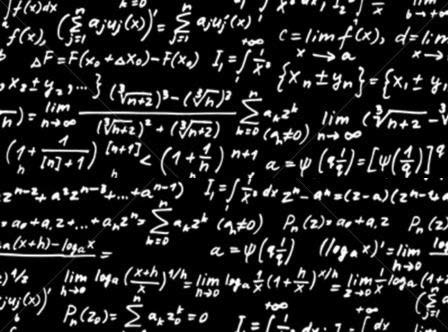
\includegraphics[width=\columnwidth]{kaavaseina.png}
	\end{figure}
	
	Perinteisissä laskareissa kiertää aluksi
	lista, johon osallistujat merkitsevät tekemänsä
	tehtävät. Nyrkkisääntö on, että
	tehtävän voi rastittaa tehdyksi, jos on tosissaan
	yrittänyt ratkaista sitä ja on valmis
	esittämään ratkaisunsa tai yrityksensä.
	Eri ihmisillä on kuitenkin huomattavasti toisistaan
	poikkeavia käsityksiä siitä, mikä tulkitaan
	yritykseksi. Järkevintä onkin toimia
	omantuntonsa mukaan, jos sellainen löytyy.
	Laskareiden pitäjä määrää jokaiselle
	tehtävälle yhden tai useamman esittäjän,
	joille annetaan jonkin aikaa keskustella
	ratkaisuistaan ja valmistautua niiden esittämiseen,
	minkä jälkeen ratkaisut esitetään
	luokan edessä. Käytännöt poikkeavat niin
	kurssikohtaisesti kuin laskareiden vetäjienkin
	kesken. Myös verkkopalautuksia hyödynnetään nykyään monilla kursseilla.
	
	Harjoitustyön sisältävät kurssit ovat
	usein muita kursseja työläämpiä opintopistemäärään
	nähden, sillä harjoitustyö
	tulee usein luentojen ja laskareiden lisäksi
	kurssin nimellisen laajuuden siitä muuttumatta.
	
	\subsubsection*{Laboratoriotyöt}
	Tietokantasovellus
	ja Tietorakenteiden harjoitustyö
	tehdään molemmat yhden periodin aikana 
	pienehkössä ryhmässä. Ryhmiä
	on melkein joka periodissa sekä myös kesällä
	ainakin kerran. Koska tällaisen pienryhmäopetuksen
	järjestäminen on kallista,
	katsotaan esitietovaatimusten täyttymistä
	tiukemmin kuin luentokursseilla.
	
	Koska osallistujamäärä on rajoitettu pieneksi,
	labraryhmään kannattaa ilmoittautua
	ajoissa. Sitten,
	kun kerran olet päässyt ryhmään, älä jätä
	menemättä aloitusluennolle tai ensimmäiseen
	tapaamiseen (aloitustapa vaihtelee
	labrasta riippuen). Ryhmän ensimmäiseen
	tapaamiseen on pakko osallistua. Jos et aio
	suorittaa labraa varaamassasi ryhmässä,
	peruuta ilmoittautumisesi etukäteen. Saapumattomuus
	ekaan tapaamiseen ilman
	pätevää syytä katsotaan yleensä labran keskeyttämiseksi.
	
	Kurssikuvaukset varoittavat laboratoriokurssien
	keskeyttämisestä ja ryhmän aloitustilaisuudesta
	pois jäämisestä. Nämä varoitukset
	on syytä ottaa vakavasti. Koska harjoitustyöryhmien
	pitäminen on suhteellisen kallista,
	haluaa kandiohjelma pitää ryhmät täysinä ja
	keskeyttäjät niistä poissa. Jos nyt harjoitustyön
	syystä tai toisesta keskeyttää, saattaa
	kestää kauan ennen kuin seuraavan kerran
	mahtuu mukaan ryhmään. Keskeyttäjät nimittäin
	joutuvat jatkossa ilmoittautumaan
	omaan ryhmäänsä, josta pääsee kurssille
	vasta siinä tapauksessa, kun ensi kertaa ilmoittautuneet
	eivät täytä kaikkia paikkoja
	kurssilla. Tyypillisesti kesän labroissa on enemmän tilaa kuin lukukausien aikana pidettävissä.
	
	\subsubsection*{Opintojen suunnittelu}
	Kuten pysyväismääräykset toteavat, ovat LuK-tutkinto
	ja FM-tutkinto kaksi erillistä tutkintoa,
	eikä LuK-tutkintoon sidottuja opintoja
	voi hyväksikäyttää FM-tutkinnossa. Kandidaatin
	tutkinto kannattaa ottaa ulos heti,
	kun vaatimukset täyttyvät, ja jättää ylimääräiset
	opinnot maisterin tutkinnon puolelle.
	Kurssin suoritusajankohdalla ei ole väliä
	sen suhteen, mihin tutkintoon sen voi sisällyttää,
	pois lukien suoritusten vanhentuminen
	opetus\-suunnitelmien muuttumisen
	myötä. Lähinnä kurssin taso ja kokonaisuuksiin
	sopiminen vaikuttaa siihen, miten
	paljon iloa siitä tutkintoa kasatessa on.
	
	Opetussuunnitelmaa lukiessa kannattaa
	muistaa, että kysymys on aina minimivaatimuksista.
	Ylimääräisiä kursseja saa suorittaa
	ja toisia tieteenaloja lukea, vaikkei tutkinnon
	paisuminen yli 180+120~opintopisteen 
	laajuuden olekaan enää nykyään suotavaa. 
	Opetus\-suunnitelmat eivät myöskään ole 
	Jumalan sanaa. Hyvällä syyllä niistä pystyy 
	periaatteessa poikkeamaan, mutta prosessi voi 
	olla senverran raskas, että helpommalla saattaa
	päästä suorittamalla kaikki vaaditut kurssit.
	Helpointa opetus\-suunnitelmista poikkeaminen
	on silloin, kun erikoistumislinjan
	opetus\-suunnitelma puhuu vain linjan
	aihepiiriin soveltuvista kursseista. Tuolloin
	linjan vastuuprofessori kyllä hyväksyy
	käytännössä minkä tahansa järkevän kokoelman
	kursseja, kunhan vain osaa perustella
	valintansa ja osoittaa, että kootut tiedot
	riittävät gradusta selviämiseen.
	
	\subsubsection*{Kandidaatin tutkinnon opinnot (LuK)}
	Kurssien välillä on
	paljon riippuvuuksia, joita on syytä pyrkiä
	noudattamaan. Nämä riippuvuudet sanelevat
	pitkälti sen, missä järjestyksessä ja
	milloin kurssit tulee suorittaa. Myös valinnaisilla
	kursseilla on vielä tässä vaiheessa
	varsin hyvin määritellyt esitietovaatimukset,
	jotka sijoittavat kurssit mallilukujärjestyksessä
	toiseen ja kolmanteen opiskeluvuoteen.
	
	Ensimmäisenä opiskeluvuonna kannattaa
	keskittyä oman koulutusohjelman opintoihin sekä pakollisten matikan tai tilastotieteen kurssien kasaamiseen.
	Näin saa molempien opinnot hyvään
	vauhtiin heti alusta alkaen. Pakollista toisen koulutusohjelman opintokokonaisuutta kannattaa miettiä
	alusta alkaen, sillä niiden opinnot kannattaa
	aloittaa jo toisena opiskeluvuonna, jos haluaa
	valmistua kandiksi kolmessa vuodessa.
	
	\subsubsection*{Maisterin tutkinnon opinnot (FM)}
	Maisterin tutkinnossa pakollisia kursseja
	on huomattavasti vähemmän kuin
	kandidaatin tutkinnossa, joten omien valintojen
	merkitys korostuu. Kannattaa siis
	miettiä, mitä todella haluaa opiskella, sekä
	ottaa selvää, millaista opetusta on lähiaikoina
	tarjolla. FM-tutkinnossa on tilaa niin
	ylimääräisille aineopintojen valinnaisille
	kursseille, oman koulutusohjelman ulkopuolisille
	kuin varsinaisille syventäville opinnoillekin.
	Gradun aloitusta ei kannata lykätä loputtomiin,
	mutta ei sen aloittamista reilun vuoden jälkeen
	tule myöskään pitää kiveen kirjoitettuna
	sääntönä.
	
	Maisterin tutkintoon tulevia opintoja voi
	suorittaa jo ennen kuin kandidaatin tutkinto
	on valmis. Näin kannattaa tehdä etenkin
	keskeisten tai harvoin luennoitavien kurssien
	kohdalla, mutta tietenkin vain silloin,
	kun näiden kurssien tosiasialliset esitiedot
	ovat jo hallussa. Kandidaatin tutkinto kannattaa
	kuitenkin suorittaa alta pois ripeästi;
	esimerkiksi seminaarien käymiseen vaaditaan
	käytännössä esitietojen puolesta Tieteellisen
	kirjoittamisen kurssin läpäiseminen.
	
	Opetussuunnitelma suosittelee varsin tiukkaa
	aikataulua FM-tutkinnon suorittamiseen.
	Tässä vaiheessa suosituksista kuitenkin
	kannattaa pyristellä irti, ellei ole aikeissa
	suorittaa ns.\,putkitutkintoa. Minimivaatimukset
	ovat todellakin vain minimivaatimuksia,
	ne täyttämällä ei vielä osaa kovinkaan
	paljon, vaan ainoastaan saa valmiudet
	opiskella alaa lisää. Yliopisto tarjoaa erinomaiset
	mahdollisuudet opiskella monia
	eri aloja järkevissä ja tasapainoisissa kokonaisuuksissa
	niin syvälle kuin vain haluaa,
	eikä toista tällaista tilaisuutta yliopiston
	ulkopuolella yleensä enää tule. Ei siis kannata
	päästää opinto-oikeudestaan irti, jos
	opiskelu vielä maistuu, vaikka olisikin jo
	polvia myöten työelämässä.
	
	\begin{figure}[b]
		\centering
		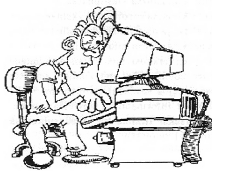
\includegraphics[width=\columnwidth]{ruuduntuijotus.png}
	\end{figure}
	
	\subsection*{Opetus ja opiskelu}
	\subsubsection*{Arvosanat}
	Tärkeintä opinnoissa ei ole mahdollisimman
	hyvien arvosanojen metsästys,
	mikä tuoreen ylioppilaan on usein jostain
	syystä vaikea ymmärtää. Jos yrittää saada
	joka kurssista nelosen tai vitosen, opiskelutahti
	alkaa mitä todennäköisimmin ennen
	pitkää kärsiä. Ensisijaisen tavoitteen tulee
	olla, että opinnot etenevät; huonoja arvosanoja
	voi (Ohjelmistotuotantoprojektia ja
	Tieteellistä kirjoittamista lukuun ottamatta)
	käydä aina korottamassa, jos siihen kokee
	jotain tarvetta. Arvosanojen perään harvemmin
	työelämässä kuulutetaan, reilusti
	venynyttä tutkinnon suorittamisaikaa voi
	sen sijaan joutua selittelemään.
	
	Monilla perus- ja aineopintojen kursseilla
	vitosenkin voi saada suhteellisen
	helposti. Hyvät arvosanat kannattaa tietysti
	ottaa vastaan niin kauan kuin kokee että
	niitä ``ilmaiseksi jaellaan'', mutta kursseja ei 
	kannata missään nimessä alkaa dropata sen takia, 
	että haluaisi saada jostain kurssista vitosen. 
	TKT:n opiskelijoiden keskuudessa
	kuultu vitsi on, että käpistelijöillä arvosanatkin
	ovat binääriä: ykköstä ja nollaa.
	
	Käytännössä matka hylätystä ykköseen
	on huomattavasti pitempi kuin matka ykkösestä
	vitoseen. Lisäksi arvosana riippuu
	edelleen hyvin pitkälti kokeesta suoriutumisesta.
	Tenttikerratkin ovat yksilöitä ja
	välillä huomaakin, että arvosanat 1--5 riippuvat
	enemmän tuurista kuin osaamisesta.
	
	\subsubsection*{Kurssipalaute}
	Kurssipalautetta kannattaa antaa jokaisesta
	kurssista, jolla tulee opintojensa aikana
	käytyä. Palautetta kannattaa antaa jo
	kurssin kuluessa, jos kurssin järjestelyissä
	tms.\,tuntuu olevan jotain huomautettavaa.
	Kurssipalautelomake löytyy
	Opiskelu-pääsivulta. Annettu palaute lähetetään
	edelleen laskariohjaajille, luennoijille
	ja kandiohjelman johtoportaalle. Palautteen
	antaminen ei ole koskaan turhaa. TKT:llä
	toimii opiskelijoiden ja henkilökunnan
	yhteistyö opetuksen kehittämisen
	osalta erinomaisesti. TKO-älyn opintovastaavien
	puoleen tulee kääntyä epäkohdissa
	koska tahansa. Opintovastaavat ovat saaneet
	toiminnastaan paljon kiitosta.
	\begin{figure}[b]
		\centering
		
\includegraphics[width=\columnwidth]{kana.png}
	\end{figure}
	
	\subsubsection*{Työssäkäynti}
	Työssäkäynti lukukausien aikana viivästyttää
	opintoja ja saattaa jopa vieraannuttaa
	yliopistosta niin, että opinnot käytännössä
	keskeytyvät. Toisaalta pelkällä opintotuella
	ja kesätöillä ei vielä kovin mukavasti elä,
	joten töissä käynti saattaa olla välttämätöntä,
	jos haluaa myös elää eikä vain opiskella.
	Alan töissä käynti usein myös lisää opiskelumotivaatiota,
	kun näkee opiskelemistaan
	asioista muitakin puolia kuin vain sen, mitä
	kurssit opettavat. Opintojen alkuvaiheessa
	kannattaa kuitenkin pyrkiä opiskelemaan
	kokopäiväisesti, sillä myöhemmin opintoihin
	mukaan pääseminen on vaikeampaa. 
	``Välivuodet'' ovat koituneet monelle
	opiskelijalle sudenkuopaksi; kannattaa
	harkita useampaan kertaan ennen
	kuin lähtee moista toteuttamaan.
	
	\vspace{0.5cm}
	\noindent\textsc{Anssi Syrjäsalo}\\
	\textsc{Piia Hartikka}
	
	\twocolumn[\section{TKT:n kursseja} {\small \itshape TKO-älyn ylläpitämässä fuksiwikissä on runsaasti tietojen\-käsittely\-tieteen kurssi\-kuvauksia.\\ \textless\url{http://fuksiwiki.tko-aly.fi}\textgreater}\vspace{0.5cm}]
	
	\subsection*{Perusopinnot}
	
	\subsubsection*{Johdatus tietojen\-käsittely\-tieteeseen (5~op)}
	Kurssin tarkoitus on johdatella tietojen\-käsittely\-tieteen
	ihmeelliseen maailmaan.
	Luentojen lisäksi luetaan artikkeleita ja kirjoitetaan
	esseitä. Syksyllä kurssin yhteydessä suoritetaan
	myös englannin kieli (4~op) ja opiskelutekniikka
	(2~op).
	
	\subsubsection*{Ohjelmoinnin perusteet (5~op)}
	Tällä kurssilla opetetaan Java-ohjelmointia
	alkeista lähtien. Sinun ei siis tarvitse
	osata valmiiksi mitään. Opetus on
	pajamuotoista, eli oppiminen tapahtuu
	tekemällä runsaasti ohjelmointitehtäviä.
	Niiden tekemiseen on tietokoneluokassa
	tarjolla apua ja ohjausta annettuina aikoina.
	Syksyllä on lisäksi luentoja. Vinkki: ohjelmoimaan
	oppii vain ohjelmoimalla, joten
	kannattaa tehdä mahdollisimman paljon
	tehtäviä! Kurssi järjestetään kaksi kertaa
	vuodessa sekä kesällä.
	
	\subsubsection*{Ohjelmoinnin jatkokurssi (5~op)}
	Nimensä mukaisesti kurssilla jatketaan
	siitä, mihin ohjelmoinnin perusteella jäätiin.
	Opetus järjestetään samaan tapaan.
	Perusasioiden ollessa hallussa harjoitustehtävien
	ohjelmat laajenevat ja tulevat entistä
	mielenkiintoisemmiksi -- ja haastavammiksi.
	Ohjelmoinnin jatkokurssin jälkeen opiskelija
	pystyy ohjelmoimaan itsenäisesti ja
	hyödyntämään internetiä ohjelmointitaitojensa
	kehittämisessä.
	\begin{figure}[b]
		\centering
		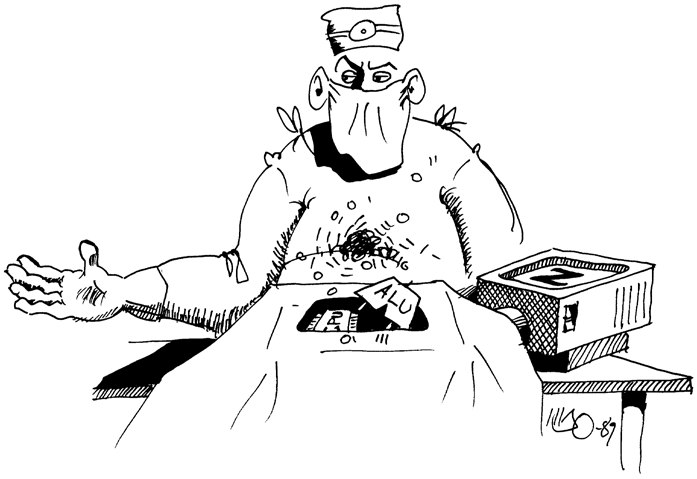
\includegraphics[width=\columnwidth]{alutohtori.png}
	\end{figure}
	
	\subsubsection*{Tietokantojen perusteet (5~op)}
	Tämä kurssi on perusopinnoista haastavin.
	Kurssiin sisältyy luentojen ja laskarien
	lisäksi tehtäviä SQL-kyselykielestä ja
	ryhmätyö, jossa suunnitellaan tietokanta.
	Kurssin vaikein aihe on relaatioalgebra,
	joka kalskahtaa ikävästi matematiikalle.
	Johdatus yliopisto\-matematiikkaan kannattaa
	olla käytynä ennen tätä kurssia.
	
	\vspace{0.5cm}
	\noindent\textsc{Piia Hartikka}
	
	\subsubsection*{Tietokoneen toiminta (5~op)}
	Kurssilla opitaan perusteet siitä, mitä tietokoneen sisällä oikeasti tapahtuu, eli tutustutaan mm.\,prosessorin toimintoihin, yhden ohjelman suoritukseen koneessa ja opetellaan hiukan symbolista kone\-kieltä. Tällä kone\-kielellä tosin ei ole kovinkaan paljon tekemistä ``oikeiden assemblerien'' (Masm, Nasm, Fasm) kanssa vaan kurssilla käytetään kandi\-ohjelman omaan opetus\-käyttöön väsättyä TTK91-assemblyä ja Titokone-simulaattoria. Pääpaino on kuitenkin enemmän teorian ymmärtämisessä. Kurssin sisältö jakaa opiskelijoita ehkä selvimmin kahteen leiriin: niihin jotka hehkuttavat ja niihin jotka vihaavat yli kaiken.
	
	\subsection*{Aineopintoja}
	\subsubsection*{Tietorakenteet ja algoritmit (10~op)}
	Kavereiden kesken Tira. Tällä kurssilla opetetaan lukuisia toinen toistaan näppärämpiä keinoja hallita tieto\-alkiota. Oikeastaan vasta kurssin asiat hallittuaan voi sanoa oikeasti osaavansa koodata. Tieto\-rakenteet ja algoritmit on myös ensimmäisiä peruskursseja, joilla kurkistetaan tietojen\-käsittelyn teoreettisempaan puoleen (algoritmit ja niiden analysointi). 
	\subsubsection*{Ohjelmistotekniikka (5~op)}
	Kurssilla annetaan perustiedot ohjelmistojen mallintamisessa käytetyistä työkaluista. Kurssilla piirretään ja luetaan kaavioita jotka kuvaavat ohjelman korkean tason rakennetta. Lisäksi opetukseen sisältyy testausta ja versionhallintaa, jotka ovat tärkeitä ohjelmointityön apuvälineitä. Tällä kurssilla tehdään myös ensimmäinen oma kokonainen ohjelmistoprojekti.
	\begin{figure}
		\centering
		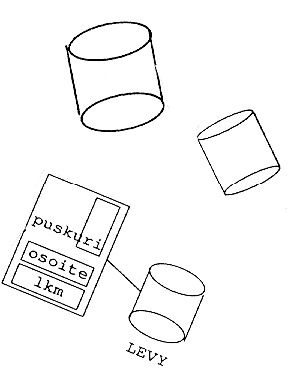
\includegraphics[width=0.8\columnwidth]{puskuriosoite.png}
	\end{figure}
	
	\subsubsection*{Käyttöjärjestelmät (5~op)}
	Kurssin voi käsittää siltana Tietokoneen toiminta "-kurssin ja Ohjelmoinnin perusteet "-kurssin välillä. Käsiteltävät asiat sisältävät käyttö\-järjestelmien rakenteen ja toimintaperiaatteet, rinnakkaisuuden toteutuksia ja ongelmia, muistinhallintaa ja virtuaalimuistia, prosessorin vuoronantoa jne.
	
	\subsubsection*{Tietoliikenteen perusteet (5~op)}
	Kurssilla paneudutaan internetin peruskäsitteistöön ja "-tekniikoihin. Kurssi etenee opettelemalla TCP/IP-pinoa taso tasolta. Tutuksi tulee siis pääpiirteittäin kaikki WWW-selaimen sielunelämästä aina verkkokortin bittitasolle asti. Kurssi antaa hyvät perustiedot tietoliikenteestä, jotka ovat tarpeen kaikkien eri linjojen opiskelijoille.
	
	Kurssin sisältö on huomattavan laaja ja yksityiskohtainen. Opiskelu perustuu paljolti TCP/IP-pinon kerrosten ja mekanismien toiminnan ulkoa opettelemiseen (esim.\,TCP-ruuhkanhallintamekanismit). Kokeessa ongelmaksi saattaa koitua hahmottaa, millä tasolla, ja kuinka yleinen vastaus kysymykseen halutaan (kokeessa saatetaan esimerkiksi kysyä, mitä tapahtuu kun opiskelija klikkaa linkkiä selaimellaan). Mikäli kurssilla vastaan tuleva lyhenteiden ja käsitteistön määrä alkaa hirvittää, kurssilla käytettävä kurssikirja on mitä mainion apu pelon\-lievitykseen.
	
	Varoitettakoon, että asioiden ja detaljien suuresta määrästä johtuen kurssista on melko vaikea saada täyttä arvosanaa. 
	
	\begin{figure*}[!b]
		\centering
		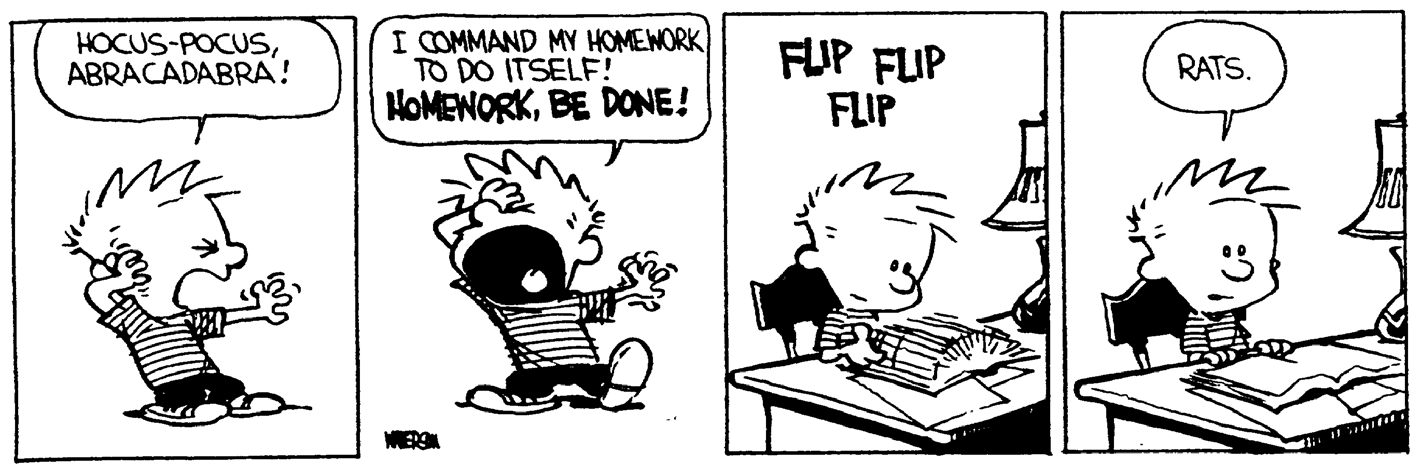
\includegraphics[width=\textwidth]{homework.png}
	\end{figure*}
\end{document}

